\documentclass[11pt]{article}
\usepackage[margin=1in]{geometry}
\usepackage[utf8]{inputenc}
\usepackage{amsmath,amssymb}
\usepackage{booktabs,array,multirow}
\usepackage{graphicx}
\usepackage[font=small,labelfont=bf]{caption}
\usepackage[round,authoryear]{natbib}
\usepackage{enumitem}
\usepackage{microtype}
\usepackage{xcolor}
\usepackage{algorithm}
\usepackage{algpseudocode}
\usepackage{tikz}
\usetikzlibrary{arrows.meta,positioning,shapes.geometric}
\usepackage[colorlinks=true,linkcolor=blue!50!black,citecolor=blue!50!black,urlcolor=blue!50!black]{hyperref}
\newcommand{\doi}[1]{\href{https://doi.org/#1}{doi:#1}}
\setlength{\parskip}{0.4em}
\newcommand{\LPRI}{\mathrm{LPRI}}
\newcommand{\LCL}{\mathrm{LCL}}
\newcommand{\tok}[1]{\textsc{#1}}

\title{Toward a Credible, Accurate and Precise Measurement System for LLM Analytical Errors and Hallucination: Statistical Process Monitoring with CUSUM, EWMA and a Process Reliability Index\\[0.3em]
\large A Protocol and Pilot Study on Industrial Quality Data}
\author{Srija Bhattacharyya\\[0.1em]
\small \href{mailto:srija.bhattacharyya04@gmail.com}{\texttt{srija.bhattacharyya04@gmail.com}}\\[0.2em]
\small B.Tech, Computer Science and Engineering, KIIT University, Bhubaneswar, India\\
\small Under the guidance of Dr Subrata Rath, Head, SQC \& OR Unit, Indian Statistical Institute, Pune}
\date{November 2026\\[0.3em]\small Preprint, version 1. Not peer reviewed.}

\begin{document}
\maketitle

\begin{abstract}
\noindent Large language models (LLMs) used for operational decisions frequently make analytical errors or hallucinate when interpreting quantitative data, producing fluent, confident statements the data do not support. Safeguards such as human review and retrieval-augmented generation reduce risk but cost effort, computation and latency, and benchmark scores, the most systematic classical method, say little about whether a model gets each calculation right. Statistical process control (SPC) offers a complementary approach: it separates routine variation from real deterioration, directing scarce oversight where it is needed.\par\smallskip\noindent We treat an LLM doing statistical analysis as a production process and build a measurement system for it, designed to be accurate, precise and credible. Each response is audited claim by claim against independently calculated references and labelled defective or not. Batches are monitored with an upper cumulative-sum (CUSUM) chart on the defect proportion and an exponentially weighted moving-average chart on an LLM Process Reliability Index. In a pilot, three LLMs analysed three Six Sigma datasets five times each. Defect rates ranged from 1 in 15 to 4 in 13 responses, with overlapping intervals. Five responses repeated one counting error near a control limit, and a dated reanalysis traced apparent instability in one dataset to pooled improvement stages. By simulation, the pilot CUSUM gives a false alarm about once every 114 in-control batches and detects a tripling of the defect rate in about six.\par\smallskip\noindent The audit was unblinded and partly self-evaluated, so the results demonstrate the method, not drift or model ranking. We pre-specify a blinded two-rater study of measurement accuracy and precision, and a Phase I calibration. As the ultimate research goal, we outline a loop in which a CUSUM signal switches the model into self-reflective retrieval (Self-RAG) only when cost and latency are justified.

\medskip\noindent\textbf{Keywords:} large language models; analytical errors; hallucination; measurement system analysis; statistical process control; CUSUM; V-mask; EWMA; process capability; inter-rater reliability; Self-RAG.
\end{abstract}

%=====================================================================
\section{Introduction}
Large language models frequently make analytical errors and hallucinate when they interpret quantitative data: they generate fluent, confident statements that are not supported by the data in front of them \citep{ji2023hallucination,huang2025survey}. Hallucination persists in state-of-the-art systems, and part of the reason lies in how models are evaluated: training and evaluation procedures that score only right-or-wrong answers reward guessing over acknowledging uncertainty \citep{kalai2025why}.

The consequences are sharper in industrial quality work than in casual use. LLMs are now asked to compute control limits, count out-of-limit points and judge process stability. A single wrong classification, such as reporting that 33 points lie below a limit when the true figure is 32, changes how a process is understood and where an improvement team looks next. For this setting the relevant question is not how accurate a model is on average, but whether a given answer can be trusted, and whether that trust holds as the model is used again and again.

This paper treats that question as a problem of measurement and process control. We build a \emph{measurement system} for LLM analytical output, require it to be accurate and precise in the sense of industrial measurement systems analysis and credible in the sense of being independently and blindly verified, and use it to feed a \emph{process-performance metric} that is monitored with classical control charts. The pilot reported here applies the system to three Six Sigma datasets (forklift breakdowns, manufacturing yield and loan-disbursement days; 141 process observations), each analysed by three model labels (GPT-5.6 Luna, Claude Sonnet 5.5 and Gemini 3.8 Flash) in five fresh sessions.

Of 45 planned responses, 42 were cleanly mapped, one was ambiguously mapped and two were absent. Seven responses were materially defective. Provisional defect proportions were 2/14 for Claude (14.3\%; exact 95\% CI 1.8--42.8\%), 4/13 for Gemini (30.8\%; 9.1--61.4\%) and 1/15 for GPT (6.7\%; 0.2--31.9\%); the intervals overlap widely, so the models cannot be ranked. Five of the seven defects were the same threshold-counting mistake on the loan data. Under pre-specified illustrative parameters, the upper CUSUM chart (reference value $k=0.19$, decision interval $h=0.67$) raised no alarm, and the lower EWMA chart of the reliability index (smoothing constant $\lambda=0.20$, limit width $L=2.7$, reference mean $\mu_0=90$) signalled once, for Claude at Run~1. By simulation, the CUSUM design has an in-control average run length of about 114 batches at a 10\% defect rate and detects a shift to 30\% in about six batches. A dated reanalysis of the loan data shows that seven apparent out-of-limit points in the Analyse \& Improve phase disappear once that phase is split at its three recorded interventions.

The contributions are:
\begin{enumerate}[leftmargin=*]
\item \textbf{A measurement system for LLM analytical errors and hallucination} with explicit criteria for accuracy, precision and credibility, mapped onto attribute measurement systems analysis \citep{aiag2010msa} and inter-rater agreement \citep{cohen1960,byrt1993}.
\item \textbf{A process-performance metric and monitoring scheme}: a binary response-level defect label, a composite LLM Process Reliability Index (LPRI), an upper CUSUM in tabular and V-mask form, and a lower EWMA, with run-length properties characterised by simulation.
\item \textbf{A pilot demonstration} with every reference value, label and chart computation reported, and a pre-specified blinded rating study and Phase~I calibration design.
\item \textbf{An ultimate research goal}: a closed loop in which a CUSUM signal switches the model into a self-reflective retrieval mode \citep{asai2024selfrag}, after which the chart is recalibrated, so that additional cost and latency are incurred only when a shift has been detected.
\end{enumerate}

Section~\ref{sec:background} reviews the concepts the system is built on. Section~\ref{sec:related} surveys present evaluation methods and their limits. Section~\ref{sec:novelty} states what this work adds. Sections~\ref{sec:methods}--\ref{sec:kappa} give the methods, reference analysis, results and measurement-system validation plan. Section~\ref{sec:goal} sets out the closed-loop research goal, followed by discussion, limitations and conclusions.

%=====================================================================
\section{Background}\label{sec:background}

\subsection{Hallucination in LLM interpretation of data}
Following \citet{ji2023hallucination} and \citet{huang2025survey}, we use \emph{hallucination} for content that is fabricated or unsupported by the available evidence. When an LLM interprets a dataset, hallucination takes concrete forms: an invented specification limit, a p-value that was never computed, a causal claim the design cannot support. Ordinary calculation and counting mistakes are related but distinct, and our rubric scores them separately (Section~\ref{sec:rubric}). \citet{kalai2025why} argue that hallucinations arise naturally from the statistics of pre-training and persist because accuracy-only evaluation penalises abstention. Hallucination is therefore a property of the model \emph{and} of how it is measured, which motivates treating measurement as a first-class design problem.

\subsection{Measurement systems: accuracy, precision and credibility}
In industrial quality practice, no process metric is trusted until the measurement system that produces it has been qualified \citep{aiag2010msa}. Three properties matter:
\begin{itemize}[leftmargin=*]
\item \textbf{Accuracy (bias):} closeness of measurements to a reference value. For a binary defect label, accuracy is agreement with an adjudicated reference label; for the answer key, it is exact agreement of reference values with the raw data.
\item \textbf{Precision:} closeness of repeated measurements to one another, split into \emph{repeatability} (the same appraiser measuring the same item twice) and \emph{reproducibility} (different appraisers measuring the same item). For attribute data, both are assessed by attribute agreement analysis, using Cohen's $\kappa$ \citep{cohen1960}, weighted $\kappa$ \citep{cohen1968} and, for more than two appraisers, Fleiss' $\kappa$ \citep{fleiss1971}.
\item \textbf{Credibility:} confidence that results are not artefacts of the procedure: independent, blinded appraisers; pre-specified decision rules; and a full audit trail.
\end{itemize}
An LLM evaluated by itself, or by an unqualified rubric, fails these tests regardless of how sophisticated the downstream statistics are.

\subsection{Process performance and statistical process control}
Once a measurement system is qualified, the quantity it produces can be treated as the output of a process and monitored. Shewhart-type charts detect large shifts; the cumulative-sum (CUSUM) chart \citep{page1954} and the exponentially weighted moving-average (EWMA) chart \citep{roberts1959,lucas1990} are the standard tools for \emph{small, persistent} shifts \citep{montgomery2019}. The CUSUM can be operated in tabular form or graphically with a V-mask, a procedure proposed by Barnard and described in the NIST/SEMATECH e-Handbook \citep{nist}; the two forms are equivalent. For a monitored proportion, Bernoulli CUSUM designs are well established \citep{reynolds1999}. When several quality characteristics are monitored jointly, as a \emph{vector}, multivariate CUSUM \citep{crosier1988} and multivariate EWMA \citep{lowry1992} charts apply.

Process \emph{capability} describes what an in-control process delivers. For attribute data, capability is expressed through the in-control fraction nonconforming rather than through Cp or Cpk \citep{montgomery2019}. A performance estimate computed before stability has been demonstrated is a \emph{performance} figure, not a capability figure; we keep that distinction throughout. Control-chart run lengths are sensitive to how in-control parameters are estimated \citep{jensen2006}, which is why the pilot parameters here are characterised by simulation rather than presented as calibrated.

\subsection{Retrieval and self-reflection}
Retrieval-augmented generation grounds an LLM's output in retrieved documents \citep{lewis2020rag}. Self-RAG \citep{asai2024selfrag} trains a model to decide \emph{when} to retrieve and to critique its own output using \emph{reflection tokens}: \tok{Retrieve} (whether to retrieve), \tok{IsRel} (whether a passage is relevant), \tok{IsSup} (whether the output is fully, partially or not supported by the passage) and \tok{IsUse} (overall usefulness, rated 1--5). Retrieval can be triggered when the probability of \tok{Retrieve}=\textit{yes} exceeds a threshold. Retrieval and critique improve factual grounding but add cost and latency to every response that uses them.

%=====================================================================
\section{Related work: present methods and their limits}\label{sec:related}

\paragraph{Static benchmarks.} Holistic suites such as HELM \citep{liang2023helm}, reasoning sets such as GSM8K \citep{cobbe2021gsm8k} and truthfulness benchmarks such as TruthfulQA \citep{lin2022truthfulqa} are the most systematic of the classical methods: they fix a test set, a scoring rule and a leaderboard. They answer ``how accurate is this model on average?'' They do not say whether a particular response is correct, they are run once rather than monitored, they carry no statement of measurement precision, and accuracy-only scoring rewards confident guessing \citep{kalai2025why}. A benchmark can rank models; it cannot remove or even track hallucination in deployment.

\paragraph{Behaviour change over time.} \citet{chen2024chatgpt} showed that the same commercial LLM service can change markedly between snapshots a few months apart, and called for continuous monitoring. Their design compared fixed snapshots; it did not provide a sequential decision rule for when a change warrants action.

\paragraph{Hallucination detectors.} SelfCheckGPT \citep{manakul2023selfcheckgpt} flags likely hallucinations by checking consistency across sampled responses, without external knowledge. FActScore \citep{min2023factscore} decomposes long-form output into atomic facts and scores the fraction supported by a knowledge source. Both work at the level of individual outputs, which our audit shares; neither specifies how detector errors are quantified as a measurement system or how scores are monitored over time.

\paragraph{LLMs as judges.} LLM judges scale cheaply but show position, verbosity and self-enhancement biases \citep{zheng2023judge}, and LLM evaluators recognise and favour their own generations \citep{panickssery2024self}. This bears directly on our pilot, whose original audit was performed by an LLM that also produced one third of the audited responses.

\paragraph{Retrieval-based mitigation.} RAG \citep{lewis2020rag} and Self-RAG \citep{asai2024selfrag} reduce hallucination by grounding generation, at a price in cost and latency. Self-RAG's retrieval decision is made token by token from the model's own probabilities; it is not driven by an externally measured, statistically monitored defect rate.

\paragraph{SPC for learning systems.} Drift detection in machine learning has long borrowed from SPC \citep{gama2014survey}, mainly for input-distribution or prediction-error streams of classifiers. Applications to the analytical correctness of generative-model outputs, with a qualified measurement system underneath, are not established.

%=====================================================================
\section{The present work and its novelty}\label{sec:novelty}

Table~\ref{tab:gap} summarises what each class of method provides. The present work combines four properties that the others provide only in part: a response-level defect measure, sequential monitoring with a formal decision rule, explicit accuracy and precision requirements for the measurement itself, and a cost-aware corrective action.

\begin{table}[!htbp]
\centering\small
\caption{Properties of present evaluation approaches and of this work. \checkmark\ = provided; $\circ$ = partly; -- = not provided.}\label{tab:gap}
\resizebox{\linewidth}{!}{\begin{tabular}{@{}lccccc@{}}
\toprule
Approach & Response-level & Over time & Decision rule & Measurement & Cost-aware \\
 & verdict & & for action & precision stated & correction \\
\midrule
Static benchmarks & -- & -- & -- & -- & -- \\
Snapshot comparison & -- & $\circ$ & -- & -- & -- \\
Detectors (SelfCheckGPT, FActScore) & \checkmark & -- & -- & $\circ$ & -- \\
LLM-as-judge & \checkmark & -- & -- & -- & -- \\
RAG / Self-RAG & $\circ$ & -- & $\circ$ & -- & $\circ$ \\
\textbf{This work} & \checkmark & $\circ$\ (pilot) & \checkmark & \checkmark\ (planned) & \checkmark\ (goal) \\
\bottomrule
\end{tabular}}
\end{table}

The novelty is fourfold. (i)~We frame the evaluation of LLM output as a \emph{measurement system} that must be shown to be accurate, precise and credible before its readings are used. (ii)~We define a \emph{process-performance metric} (the response-level defect rate and the LPRI) and monitor it with CUSUM and EWMA charts whose operating characteristics are stated. (iii)~We illustrate on DMAIC project data that claim-level auditing exposes systematic failure modes that an aggregate score would hide. (iv)~We set out a closed loop in which the CUSUM signal, not a per-token heuristic, decides when to pay for retrieval and self-critique.

%=====================================================================
\section{Materials and methods}\label{sec:methods}

\subsection{Notation}
Table~\ref{tab:notation} fixes the meaning of each symbol. The CUSUM reference value $k$ and Cohen's agreement coefficient $\kappa$ (Greek kappa) are unrelated quantities.

\begin{table}[!htbp]
\centering\small
\caption{Notation.}\label{tab:notation}
\begin{tabular}{@{}l p{0.6\linewidth} l@{}}
\toprule
Symbol & Meaning & Value used \\
\midrule
$t$ & Run (batch) index, $t=1,\dots,5$ & -- \\
$D_t$ & Proportion of materially defective responses in batch $t$ & data \\
$I_t$ & Proportion of data-integrity events (missing or ambiguous responses) in batch $t$ & data \\
$p_0$ & Acceptable (in-control) per-response defect probability & 0.10 \\
$p_1$ & Defect probability the CUSUM is designed to detect & 0.30 \\
$k$ & CUSUM reference value (allowance) & 0.19 \\
$h$ & CUSUM decision interval; signal when $S_t>h$ & 0.67 \\
$d,\ \theta$ & V-mask lead distance and half-angle & $d=3.53$ \\
$S_t$ & Upper CUSUM statistic & computed \\
$\lambda$ & EWMA smoothing constant & 0.20 \\
$L$ & EWMA control-limit width in standard deviations & 2.7 \\
$\mu_0$ & EWMA reference (target) mean of LPRI & 90 (92 in sensitivity) \\
$\sigma_0$ & In-control standard deviation of LPRI & 13.86 \\
$z_t$ & EWMA statistic & computed \\
$\kappa$ & Cohen's kappa: chance-corrected agreement between two raters & pending \\
$\kappa_w$ & Quadratically weighted kappa for the 0--3 severity score & pending \\
PABAK & Prevalence- and bias-adjusted kappa, $2p_o-1$ & pending \\
\bottomrule
\end{tabular}
\end{table}

\subsection{Datasets}
Three DMAIC project datasets were used, each split into improvement phases (Table~\ref{tab:datasets}). The 141 observations are process data, not LLM trials.

\begin{table}[!htbp]
\centering\small
\caption{Process datasets.}\label{tab:datasets}
\begin{tabular}{@{}l p{0.38\linewidth} l r@{}}
\toprule
Dataset & Measure & Phases ($n$) & Total \\
\midrule
Forklift breakdown & Breakdowns per 15-day period; target strictly $<3$ & 15 / 19 / 13 & 47 \\
Manufacturing yield & \% yield per production experiment & 10 / 8 / 7 & 25 \\
Loan disbursement & Days to disburse, one value per month & 26 / 36 / 7 & 69 \\
\bottomrule
\multicolumn{4}{@{}l}{\footnotesize Phases: Baseline / Analyse \& Improve (Improve for yield) / Control.}
\end{tabular}
\end{table}

The source workbook holds more than the prompts passed on. It dates each loan observation monthly (October 2019 to June 2025), places the three intervention notes on specific months, and records a second loan column labelled ``No of Loan application'' (values of 23--38 million, so probably a monetary amount rather than a count). The yield sheet numbers its 25 experiments and records raw-material and additive masses, but not the yield formula. None of this was given to the models; it is used only in the reference reanalysis (Section~\ref{sec:loan-dated}).

\subsection{Models, prompts and collection}
Three model labels were tested as displayed in their chat interfaces: GPT-5.6 Luna, Claude Sonnet 5.5 and Gemini 3.8 Flash. Build identifiers, sampling parameters and system prompts were not recorded. Each model received one standardised prompt per dataset (Appendix~\ref{app:prompts}, verbatim) in a fresh chat for each of five runs: $3\times3\times5=45$ planned responses. Fresh chats reduce carry-over but do not guarantee independence. The loan prompt listed the three intervention annotations but not the month of each observation, so a model could not map interventions to observations.

\subsection{The measurement system: reference values and audit rubric}\label{sec:rubric}
\textbf{Reference values (the answer key).} Every reference value was computed from the raw workbook and re-computed independently in code (Section~\ref{sec:reference}). This establishes the accuracy of the standard against which responses are measured.

\textbf{Rubric.} Each claim in a response is scored 0 (correct and supported), 1 (minor imprecision with no material effect), 2 (material error: a wrong statistic, count, limit classification or interpretation) or 3 (fabricated or high-impact unsupported claim, i.e.\ hallucination in the strict sense). A response is \emph{materially defective} if any claim scores 2 or 3. Missing responses, duplicate uploads and ambiguous prompt--response mappings are \emph{data-integrity events}, recorded separately and never counted as defects.

\textbf{Deviation from the original audit.} The original audit counted one ambiguous Claude Run~3 slot (a forklift prompt followed by a loan analysis) as a provisional defect, contrary to the integrity rule. This version reclassifies it as an integrity event; the original classification is reported as a sensitivity analysis (Section~\ref{sec:sensitivity}).

\textbf{Measurement-system qualification.} Table~\ref{tab:msa} maps the requirements of attribute measurement systems analysis onto this rubric. Only the accuracy of the answer key is established in this version; the remaining properties are assessed by the pre-specified study in Section~\ref{sec:kappa}.

\begin{table}[!htbp]
\centering\small
\caption{Measurement-system requirements and their status.}\label{tab:msa}
\begin{tabular}{@{}p{0.17\linewidth} p{0.42\linewidth} p{0.3\linewidth}@{}}
\toprule
Property & How it is assessed & Status in this version \\
\midrule
Accuracy of the standard & Reference values recomputed independently in code & Established \\
Accuracy of labels (bias) & Agreement of each rater, and of the original LLM audit, with the adjudicated label & Pending (Section~\ref{sec:kappa}) \\
Repeatability & Each rater re-scores a random subset after a washout period; within-rater $\kappa$ & Pending \\
Reproducibility & Two blinded raters; between-rater $\kappa$, $\kappa_w$, PABAK & Pending \\
Credibility & Blinding, randomised order, pre-specified decision rule, retained raw ratings & Protocol fixed \\
\bottomrule
\end{tabular}
\end{table}

\subsection{Process-performance metrics: batches and LPRI}
For each model, run $t$ is one batch of three planned responses, one per dataset. With $d_t$ defective responses and $m_t$ integrity events in the batch,
\begin{equation}
D_t=\frac{d_t}{3},\qquad I_t=\frac{m_t}{3},\qquad \LPRI_t=100\left(1-0.8\,D_t-0.2\,I_t\right).
\label{eq:lpri}
\end{equation}
Both proportions use the planned batch size of three, so a batch with one missing response and one defect has $D_t=0.333$, not $0.5$; the missing slot is penalised through $I_t$ instead. The weights 0.8 and 0.2 are hypotheses to be validated, not estimates.

The underlying process-performance parameter is the per-response defect probability $p$. Its capability counterpart is the in-control value $p_0$, estimable only after a stable Phase~I. When the number of audited claims per response is recorded, the same data also yield defects per opportunity (claims as opportunities) and hence DPMO.

\subsection{CUSUM chart: tabular and V-mask forms}
An upper one-sided CUSUM on $D_t$ detects a small, sustained rise in defects:
\begin{equation}
S_t=\max\left(0,\;S_{t-1}+D_t-k\right),\qquad S_0=0,\qquad \text{signal if } S_t>h.
\label{eq:cusum}
\end{equation}
The reference value $k$ is the Bernoulli log-likelihood-ratio allowance for an acceptable defect probability $p_0=0.10$ and a rate worth detecting $p_1=0.30$ \citep{reynolds1999}:
\begin{equation}
k=\frac{\ln\!\left[(1-p_0)/(1-p_1)\right]}{\ln(p_1/p_0)+\ln\!\left[(1-p_0)/(1-p_1)\right]}
=\frac{0.2513}{1.0986+0.2513}=0.186\approx0.19.
\label{eq:k}
\end{equation}
The decision interval $h=0.67$ was fixed before any chart was computed. Neither $k$ nor $h$ was estimated from an in-control baseline.

\textbf{V-mask form.} The same scheme can be read graphically. Plot the cumulative defect proportion $T_t=\sum_{i\le t}D_i$ and place a V-shaped mask with its vertex a lead distance $d$ ahead of the latest point; a shift is signalled if any earlier point falls below the lower arm. Algebraically the tabular chart signals at batch $t$ exactly when, for some earlier batch $j$,
\begin{equation}
T_t-T_j>h+k\,(t-j),
\label{eq:vmask-cond}
\end{equation}
which is the V-mask condition with arm slope $k$. The two parameterisations are related by
\begin{equation}
d=\frac{h}{k},\qquad \theta=\arctan\!\left(\frac{k}{a}\right),
\label{eq:vmask}
\end{equation}
where $\theta$ is the half-angle of the mask and $a$ the plotting aspect ratio (vertical units per batch) \citep{nist}. Here $d=0.67/0.19=3.53$ batches.

In context, Eq.~\ref{eq:vmask-cond} says what pattern of defects the chart treats as a shift. A single batch with all three responses defective signals at once ($1-0.19=0.81>0.67$). A single batch with two defects does not ($0.667-0.19=0.477$), but two such batches in a row do ($1.333-0.38=0.953$). One defect per batch, the pattern Gemini showed in its last three runs, signals only after five consecutive batches ($1.667-0.95=0.717$). The chart is therefore built to catch small, persistent shifts while tolerating isolated bad batches.

\subsection{EWMA chart}
A lower one-sided EWMA on LPRI detects a sustained fall in reliability \citep{roberts1959,lucas1990}:
\begin{equation}
z_t=\lambda\,\LPRI_t+(1-\lambda)\,z_{t-1},\qquad z_0=\mu_0,
\label{eq:ewma}
\end{equation}
\begin{equation}
\LCL_t=\mu_0-L\,\sigma_0\sqrt{\frac{\lambda}{2-\lambda}\left[1-(1-\lambda)^{2t}\right]},
\label{eq:lcl}
\end{equation}
with $\lambda=0.20$, $L=2.7$ and $\mu_0=90$. The standard deviation is the LPRI standard deviation implied by $p_0=0.10$ with no missing responses:
\begin{equation}
\sigma_0=100\times0.8\times\sqrt{\frac{p_0(1-p_0)}{3}}=80\times0.1732=13.86.
\label{eq:sigma}
\end{equation}
The same $p_0$ implies an in-control mean of $100(1-0.8\times0.10)=92$, not 90. The pre-specified $\mu_0=90$ is kept as the primary setting and $\mu_0=92$ is reported as a sensitivity analysis.

\subsection{Confidence intervals and run-length characterisation}
Defect proportions are reported with exact (Clopper--Pearson) 95\% intervals. The average run length (ARL), the expected number of batches before a signal, was estimated for each chart design by Monte Carlo simulation: 200{,}000 series per setting, each batch drawn as $\mathrm{Binomial}(3,p)$ defects with no missing responses, at $p=0.10$ (in control), 0.20 and 0.30. With this many replicates the Monte Carlo standard error of each ARL is below 1\% of its value.

\section{Reference analysis}\label{sec:reference}
All values below were recomputed from the raw workbook in Python and match the hand calculations used for scoring.

\subsection{Forklift breakdowns}
\begin{table}[!htbp]
\centering\small
\caption{Forklift breakdowns per 15-day period.}
\begin{tabular}{@{}lrrrrcrc@{}}
\toprule
Phase & $n$ & Mean & Median & SD & Min--Max & Var/mean & Periods $<3$ \\
\midrule
Baseline & 15 & 4.7333 & 5 & 2.1536 & 2--9 & 0.98 & 2/15 (13.3\%) \\
Analyse \& Improve & 19 & 3.8947 & 4 & 3.0165 & 0--11 & 2.34 & 6/19 (31.6\%) \\
Control & 13 & 1.3846 & 1 & 1.1209 & 0--4 & 0.91 & 11/13 (84.6\%) \\
\bottomrule
\end{tabular}
\end{table}
Mean breakdowns fell 70.75\% from Baseline to Control. The Baseline c-chart has
\begin{equation}
\mathrm{CL}=\bar c=4.7333,\qquad \mathrm{UCL}=\bar c+3\sqrt{\bar c}=11.2602,\qquad \mathrm{LCL}=\max\!\left(0,\;\bar c-3\sqrt{\bar c}\right)=0,
\end{equation}
and no Baseline point lies outside these limits. As a formal check of the Poisson equidispersion assumption, the index-of-dispersion statistic $(n-1)s^2/\bar x$, referred to $\chi^2_{n-1}$, gives two-sided $p=0.94$ for Baseline, $0.92$ for Control and $0.002$ for Analyse \& Improve, which is overdispersed as expected if its rate changed partway through. A c-chart also assumes equal exposure per period; equal 15-day intervals do not establish equal fleet size or operating hours. DPMO cannot be computed without an opportunity count.

\subsection{Manufacturing yield}
\begin{table}[!htbp]
\centering\small
\caption{Manufacturing yield (\%).}
\begin{tabular}{@{}lrrrrc@{}}
\toprule
Phase & $n$ & Mean & Median & SD & Min--Max \\
\midrule
Baseline & 10 & 7.0100 & 7.05 & 0.2025 & 6.7--7.3 \\
Improve & 8 & 8.7250 & 8.75 & 0.1982 & 8.4--9.0 \\
Control & 7 & 9.9286 & 9.90 & 0.1113 & 9.8--10.1 \\
\bottomrule
\end{tabular}
\end{table}
Mean yield rose 2.9186 percentage points (41.64\% relative) and the SD fell by about 45\%; the phase ranges do not overlap. An I-MR chart suits single measurements in run order; a p-chart would be preferable if yield is a proportion of known counts. Cp and Cpk cannot be calculated: there are no specification limits and stability has not been shown. Phase separation alone does not establish what caused the increase.

\subsection{Loan disbursement days}
Individuals (I) and moving-range (MR) limits use the average moving range $\overline{MR}$:
\begin{equation}
\mathrm{I\text{-}chart:}\ \bar x\pm2.66\,\overline{MR},\qquad \mathrm{MR\text{-}chart\ UCL}=3.267\,\overline{MR}.
\end{equation}
\begin{table}[!htbp]
\centering\small
\caption{Loan disbursement days with phase-specific I-MR limits.}
\resizebox{\linewidth}{!}{\begin{tabular}{@{}lrrrrcrccr@{}}
\toprule
Phase & $n$ & Mean & Median & SD & Min--Max & $\overline{MR}$ & I-chart LCL / UCL & MR UCL & Outside \\
\midrule
Baseline & 26 & 20.4615 & 20 & 2.6112 & 16--26 & 2.8800 & 12.80 / 28.12 & 9.41 & 0 \\
Analyse \& Improve & 36 & 10.1389 & 10.5 & 2.0305 & 7--14 & 1.1714 & 7.02 / 13.25 & 3.83 & 7 \\
Control & 7 & 7.4286 & 7 & 0.5345 & 7--8 & 0.8333 & 5.21 / 9.65 & 2.72 & 0 \\
\bottomrule
\end{tabular}}
\end{table}
Mean time fell 13.03 days (63.69\%) from Baseline to Control. Judged against its own limits, Analyse \& Improve has three points above the UCL (three 14s) and four below the LCL (four 7s). Against the Baseline LCL of 12.80, 32 of 36 Analyse \& Improve observations lie below it; four (13, 14, 14, 14) lie above. All seven Control values lie below it.

\subsection{Dated reanalysis of the loan data}\label{sec:loan-dated}
The workbook's month column shows that Analyse \& Improve is not one process but three, each beginning at a recorded intervention month (Figure~\ref{fig:loan}). Split at those months, the phase forms a staircase of 12.17, 10.17 and 8.08 days, and each stage is in control on its own I-MR limits (7.81--16.52, 7.51--12.83 and 5.67--10.50 days), with no points outside.

\begin{figure}[!htbp]
\centering
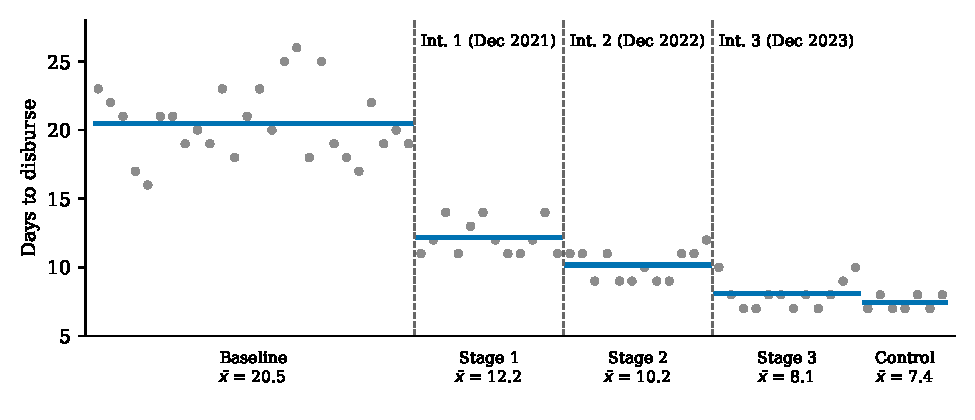
\includegraphics[width=\linewidth]{figures/loan_staircase.pdf}
\caption{Loan disbursement days by month, October 2019 to June 2025. Blue lines are stage means; dashed lines mark the three recorded intervention months. Source: process-data workbook, sheet 3.}
\label{fig:loan}
\end{figure}

This changes the interpretation in two ways. First, the seven ``violations'' in the phase-level analysis are artefacts of pooling three process levels under one set of limits. Second, each drop in level begins in the month an intervention was recorded. That timing is consistent with an effect but does not prove one: there is no control series, and any concurrent change would show the same pattern. The second loan column rose by about 52\% from Baseline to Control while disbursement time fell (Pearson $r=-0.88$), so higher volume did not lengthen processing time. The models were never given the months; their answers were scored against the phase-level reference, which is what the prompt asked for.

\section{Results}\label{sec:results}

\subsection{Response-level audit}
Forty-two of 45 planned slots held a cleanly mapped response; one was ambiguous and two were empty. Seven responses were materially defective (Table~\ref{tab:audit}).

\begin{table}[!htbp]
\centering\small
\caption{Response-level labels. 0 = no material defect; D = materially defective; -- = absent; Amb.\ = ambiguous prompt--response mapping (a data-integrity event, not a defect).}\label{tab:audit}
\begin{tabular}{@{}lcccc p{0.42\linewidth}@{}}
\toprule
Model & Run & Forklift & Yield & Loan & Notes \\
\midrule
Claude & 1 & D & 0 & D & Forklift median wrong; loan sum of squares and violation count wrong \\
Claude & 2 & 0 & 0 & 0 & One minor internal count inconsistency (score 1) \\
Claude & 3 & Amb. & 0 & 0 & Forklift slot holds a loan analysis; source of mismatch unresolved \\
Claude & 4 & 0 & 0 & 0 & \\
Claude & 5 & 0 & 0 & 0 & \\
\midrule
Gemini & 1 & 0 & 0 & D & Baseline-LCL comparison and threshold count wrong \\
Gemini & 2 & 0 & 0 & 0 & \\
Gemini & 3 & 0 & 0 & D & 33/36 below Baseline LCL (true 32/36) \\
Gemini & 4 & -- & 0 & D & Forklift response absent; threshold count wrong \\
Gemini & 5 & 0 & -- & D & Yield response absent; threshold comparison wrong \\
\midrule
GPT$^{*}$ & 1 & 0 & 0 & 0 & \\
GPT$^{*}$ & 2 & 0 & 0 & 0 & \\
GPT$^{*}$ & 3 & 0 & 0 & D & 33/36 below Baseline LCL \\
GPT$^{*}$ & 4 & 0 & 0 & 0 & Minor assumption about the loan unit (score 1) \\
GPT$^{*}$ & 5 & 0 & 0 & 0 & Wrong intermediate sums of squares, correct final SDs (score 1) \\
\bottomrule
\multicolumn{6}{@{}l}{\footnotesize $^{*}$GPT responses were scored by the same ChatGPT workflow that produced them (self-evaluation).}
\end{tabular}
\end{table}

\begin{table}[!htbp]
\centering\small
\caption{Material-defect proportions with exact (Clopper--Pearson) 95\% confidence intervals.}\label{tab:rates}
\begin{tabular}{@{}lccc@{}}
\toprule
Model & Defective / evaluable & Proportion & 95\% CI \\
\midrule
Claude Sonnet 5.5 & 2 / 14 & 14.3\% & 1.8--42.8\% \\
Gemini 3.8 Flash & 4 / 13 & 30.8\% & 9.1--61.4\% \\
GPT-5.6 Luna$^{*}$ & 1 / 15 & 6.7\% & 0.2--31.9\% \\
\bottomrule
\end{tabular}
\end{table}
Table~\ref{tab:rates} gives the defect proportions with exact confidence intervals. The intervals overlap almost entirely, so these data cannot rank the models. Six of the seven defects were on the loan dataset, one on forklift and none on yield. All seven were calculation or classification errors; none was recorded as a fabrication (score~3).

\subsection{Error patterns}
\textbf{One counting error recurred across sessions and models.} Five responses (Gemini Runs 1, 3, 4, 5; GPT Run 3) said that 33 of 36 Analyse \& Improve values lie below the Baseline LCL of 12.80. The true count is 32: one value is 13 and three are 14. A value close to a limit appears to be a trap. The prompt did not ask for this comparison; the models volunteered it.

\textbf{Right answer, wrong working.} GPT Run 5 reported correct forklift SDs after showing incorrect intermediate sums of squares. Under the rubric this scores 1, but a reader who reused the working would inherit the error.

\textbf{Appropriate caution was common.} Most responses correctly stated that improvement is not stability, that phase-specific limits can hide between-phase shifts, that Cp/Cpk need specification limits and that annotations do not prove causation. The rubric does not let these strengths offset a material numerical error.

\subsection{Batch quantities}
Table~\ref{tab:batch} gives each model's batch defect proportion $D_t$, integrity proportion $I_t$ and LPRI (Eq.~\ref{eq:lpri}). Gemini's lower mean LPRI reflects both its recurring loan error and its two absent responses.
\begin{table}[!htbp]
\centering\small
\caption{Batch defect proportion $D_t$, integrity proportion $I_t$ and $\LPRI_t$ (Eq.~\ref{eq:lpri}).}\label{tab:batch}
\begin{tabular}{@{}llcccccr@{}}
\toprule
Model & Quantity & Run 1 & Run 2 & Run 3 & Run 4 & Run 5 & Mean \\
\midrule
\multirow{2}{*}{Claude} & $D_t$ / $I_t$ & 0.667 / 0 & 0 / 0 & 0 / 0.333 & 0 / 0 & 0 / 0 & \\
 & LPRI & 46.67 & 100 & 93.33 & 100 & 100 & 88.00 \\
\multirow{2}{*}{Gemini} & $D_t$ / $I_t$ & 0.333 / 0 & 0 / 0 & 0.333 / 0 & 0.333 / 0.333 & 0.333 / 0.333 & \\
 & LPRI & 73.33 & 100 & 73.33 & 66.67 & 66.67 & 76.00 \\
\multirow{2}{*}{GPT} & $D_t$ / $I_t$ & 0 / 0 & 0 / 0 & 0.333 / 0 & 0 / 0 & 0 / 0 & \\
 & LPRI & 100 & 100 & 73.33 & 100 & 100 & 94.67 \\
\bottomrule
\end{tabular}
\end{table}

\subsection{CUSUM and EWMA charts}
Under the primary settings the CUSUM raised no alarm (Figure~\ref{fig:cusum}). Claude's statistic peaks at $S_1=0.477$ after its two-defect first batch and decays to zero. Gemini's rises steadily to $S_5=0.430$ because it has a defect in each of the last three batches, all from the same loan counting error.

\begin{figure}[!htbp]
\centering
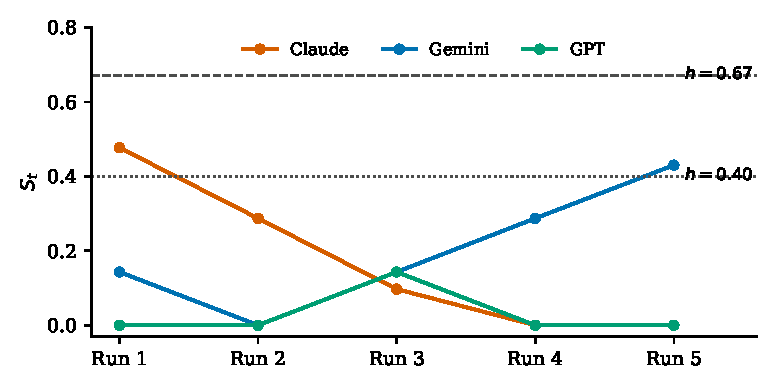
\includegraphics[width=0.78\linewidth]{figures/cusum.pdf}
\caption{Upper CUSUM of the batch defect proportion (Eq.~\ref{eq:cusum}; $k=0.19$). Dashed: decision interval $h=0.67$; dotted: sensitivity setting $h=0.40$. Runs are in recorded order, not verified time order.}
\label{fig:cusum}
\end{figure}

The EWMA signalled once (Figure~\ref{fig:ewma}): Claude at Run~1, with $z_1=81.33$ against $\LCL_1=82.52$. It then recovered. Gemini's EWMA fell from 89.33 to 79.13 and finished 0.91 points above $\LCL_5=78.21$. GPT stayed well inside the limit.

\begin{figure}[!htbp]
\centering
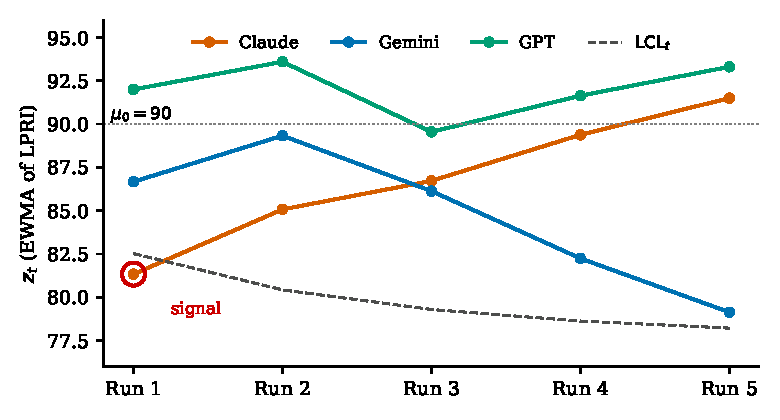
\includegraphics[width=0.78\linewidth]{figures/ewma.pdf}
\caption{Lower EWMA of LPRI (Eqs.~\ref{eq:ewma}--\ref{eq:lcl}; $\lambda=0.20$, $L=2.7$, $\mu_0=90$, $\sigma_0=13.86$) with the time-varying lower control limit.}
\label{fig:ewma}
\end{figure}

\subsection{Sensitivity of the alarm pattern}\label{sec:sensitivity}
\begin{table}[!htbp]
\centering\small
\caption{Signals under alternative analyst choices.}\label{tab:sens}
\begin{tabular}{@{}p{0.42\linewidth}p{0.26\linewidth}p{0.22\linewidth}@{}}
\toprule
Setting changed & CUSUM signals & EWMA signals \\
\midrule
None (primary analysis) & none & Claude R1 \\
Tighter decision interval, $h=0.40$ & Claude R1; Gemini R5 & Claude R1 \\
EWMA reference mean $\mu_0=92$ & none & Claude R1; Gemini R5 \\
Original audit: Claude R3 ambiguous slot counted as a defect & none (Claude R1, R3 at $h=0.40$) & Claude R1 \\
Gemini R4--R5 defects divided by responses received (2) & Gemini R5 ($S_5=0.763$) & Claude R1; Gemini R5 \\
\bottomrule
\end{tabular}
\end{table}
Gemini's status at Run~5 changes under three of the four alternatives (Table~\ref{tab:sens}). With five batches per model, chart verdicts are driven by analyst choices as much as by the data.

\subsection{Run-length properties of the pilot designs}
\begin{table}[!htbp]
\centering\small
\caption{Simulated average run length (batches) with batches of three and no missing responses.}\label{tab:arl}
\begin{tabular}{@{}lccc@{}}
\toprule
True defect rate $p$ & CUSUM ($k=0.19$, $h=0.67$) & EWMA, $\mu_0=90$ & EWMA, $\mu_0=92$ \\
\midrule
0.10 (in control) & 114 & 327 & 155 \\
0.20 & 15 & 19 & 14 \\
0.30 & 6.4 & 6.3 & 5.4 \\
\bottomrule
\end{tabular}
\end{table}
The pilot CUSUM gives a false alarm about once every 114 in-control batches and detects a tripling of the defect rate in about six (Table~\ref{tab:arl}). Setting $\mu_0=90$ below the in-control mean of 92 makes the EWMA conservative, roughly doubling its in-control ARL. These figures assume $p_0$ is known exactly; with $p_0$ estimated from a short Phase~I, actual run lengths can differ substantially \citep{jensen2006}.

\subsection{Process-performance estimate}\label{sec:performance}
Pooling the three models, 7 of 42 cleanly mapped responses were materially defective: $\hat p=0.167$ (exact 95\% CI 0.070--0.314). This is a \emph{performance} estimate, not a capability figure: it pools three different processes, rests on labels whose precision is not yet established, and was obtained before any in-control baseline was demonstrated. Defects per million opportunities cannot be computed because the number of audited claims per response was not recorded; the confirmatory protocol records it.

%=====================================================================
\section{Measurement-system validation: inter-rater agreement}\label{sec:kappa}
\textbf{No $\kappa$ is reported in this version, because no paired independent ratings exist yet.} Every label in Section~\ref{sec:results} comes from one unblinded LLM workflow. Treating the three models, or earlier write-ups, as ``raters'' would change the unit of analysis and give a coefficient that answers a different question. The study below is an attribute agreement analysis in the sense of \citet{aiag2010msa}, fixed before any second rating is collected; its results will be reported in a subsequent version whatever they show.

\subsection{Design}
\begin{enumerate}[leftmargin=*]
\item \textbf{Material.} The 42 cleanly mapped responses form the primary set; the ambiguous slot is rated but analysed only in a sensitivity check ($n=43$).
\item \textbf{Blinding.} Model names and self-identifying text are removed. Each response receives a random code (R01--R43) and is presented in random order. The code key is held by the author, who does not rate.
\item \textbf{Reproducibility.} Two people with SPC training who did not collect the responses rate every response independently, using the rubric and the Section~\ref{sec:reference} reference values, after calibrating on three practice responses not drawn from the study set.
\item \textbf{Repeatability.} Each rater re-scores a random subset of 12 responses, re-coded, after a washout of at least two weeks.
\item \textbf{Accuracy.} A third person, also blind to model identity, adjudicates every disagreement. The adjudicated label is the reference; each rater's and the original LLM audit's agreement with it measures bias.
\end{enumerate}

\subsection{Statistics}
For two sets of ratings with a $2\times2$ table of counts $a$ (both defective), $b$ and $c$ (disagreements) and $d$ (both not defective), $N=a+b+c+d$,
\begin{equation}
p_o=\frac{a+d}{N},\qquad p_e=\frac{(a+b)(a+c)+(c+d)(b+d)}{N^2},\qquad \kappa=\frac{p_o-p_e}{1-p_e}.
\label{eq:kappa}
\end{equation}
Here $p_o$ is observed agreement and $p_e$ is the agreement expected by chance from the marginal proportions. Because $\kappa$ can be low despite high agreement when one category dominates \citep{feinstein1990}, the prevalence- and bias-adjusted kappa \citep{byrt1993} is reported alongside it:
\begin{equation}
\mathrm{PABAK}=2p_o-1.
\label{eq:pabak}
\end{equation}
For the ordinal 0--3 severity score, the quadratically weighted kappa \citep{cohen1968} uses weights $w_{ij}=1-(i-j)^2/9$:
\begin{equation}
\kappa_w=\frac{\sum_{i,j}w_{ij}O_{ij}-\sum_{i,j}w_{ij}E_{ij}}{N-\sum_{i,j}w_{ij}E_{ij}},\qquad E_{ij}=\frac{O_{i\cdot}\,O_{\cdot j}}{N},
\label{eq:wkappa}
\end{equation}
where $O_{ij}$ is the number of responses scored $i$ by one rating and $j$ by the other. The same formulas give within-rater (repeatability), between-rater (reproducibility) and rater-versus-reference (accuracy) agreement. Confidence intervals use the percentile bootstrap with 2{,}000 resamples of responses. Agreement between the original ChatGPT audit and the adjudicated label is reported separately for GPT responses and for the others, as a direct measure of the self-preference bias documented by \citet{panickssery2024self}.

\subsection{Decision rule and expected precision}
The adjudicated labels will be used for monitoring only if between-rater binary $\kappa\ge0.60$, the threshold fixed before any rating was collected; otherwise the rubric is revised, both raters re-score, and the failed round is reported. All intervals are reported. With 42 responses and a defect prevalence near 17\%, simulation shows that a true $\kappa\approx0.70$ yields a 95\% interval about 0.55 wide, so the study will test whether the rubric is usable rather than pin down its reliability precisely.

%=====================================================================
\section{Ultimate research goal: a CUSUM-triggered Self-RAG loop}\label{sec:goal}
The pilot measures and monitors; it does not correct. The ultimate goal of this programme is a closed loop in which a detected shift triggers corrective action automatically, while cost and latency are spent only when the evidence warrants it. This section is a design proposal; none of it has been implemented or tested.

\paragraph{Two operating modes.} In \emph{standard mode} (A) the model answers directly, at per-response cost $c_A$ and latency $\ell_A$. In \emph{Self-RAG mode} (B) it retrieves supporting material on demand and critiques its own output with the reflection tokens of \citet{asai2024selfrag}, at higher cost $c_B>c_A$ and latency $\ell_B>\ell_A$. For SPC tasks the retrieval corpus would hold the raw data, the reference formulas and the organisation's control-chart standards.

\paragraph{Switching threshold.} Mode A is the default. Its defect proportion is monitored with the upper CUSUM of Eq.~\ref{eq:cusum}, designed from a Phase~I estimate of $p_{0,A}$. The CUSUM is used because the failure this loop must catch, a small persistent rise such as a recurring counting error, is exactly the shift it is designed to detect. The model switches to mode B when $S_t>h$ \emph{and} the switch is economically justified:
\begin{equation}
c_{\mathrm{def}}\,\bigl(\hat p_A-p_{0,B}\bigr)\;\ge\;c_B-c_A,
\label{eq:switch}
\end{equation}
where $c_{\mathrm{def}}$ is the expected cost of one defective response reaching a decision-maker, $\hat p_A$ is the post-shift defect rate in mode A and $p_{0,B}$ the in-control rate in mode B. A latency budget $\ell_{\max}$ caps the switch: if $\ell_B>\ell_{\max}$, the system alerts a human instead. Statistical evidence decides \emph{whether} the process has shifted; the cost criterion decides \emph{whether correcting it is worth paying for}.

\paragraph{Reflection tokens as an auxiliary measurement.} In mode B each response carries \tok{IsSup} (fully, partially or not supported) and \tok{IsUse} (1--5) tokens. A response tagged \tok{IsSup}=\textit{no support} is a candidate defect that costs nothing extra to observe. Because this is a new measurement system, its accuracy and precision against the human-adjudicated label must be established, with the same agreement statistics as Section~\ref{sec:kappa}, before it is used to drive the chart.

\paragraph{Recalibration after the threshold is crossed.} A mode switch is a process intervention, so the mode-A chart cannot simply continue. On switching, the CUSUM is reset ($S=0$) and re-designed for mode B: $p_{0,B}$ is estimated from a short Phase~I in mode B, $k$ is recomputed from Eq.~\ref{eq:k} with $p_{0,B}$ and the chosen $p_1$, and $h$ is chosen by simulation for the target in-control ARL. To decide when to return, a small number of shadow probe batches are run periodically in mode A and monitored with their own CUSUM; the system returns to mode A when that CUSUM has stayed below its limit for a pre-set number of probes and the economic condition of Eq.~\ref{eq:switch} no longer holds.

\paragraph{Monitoring a vector of outputs.} Once cost and latency are part of the decision, the monitored quantity becomes a vector, $\mathbf{x}_t=(D_t,\,I_t,\,\bar c_t,\,\bar\ell_t)$: defect rate, integrity rate, mean cost and mean latency per batch. Multivariate CUSUM \citep{crosier1988} and multivariate EWMA \citep{lowry1992} charts monitor such vectors jointly while accounting for correlation between the components.

Figure~\ref{fig:loop} and Algorithm~\ref{alg:loop} summarise the loop.

\begin{figure}[!htbp]
\centering
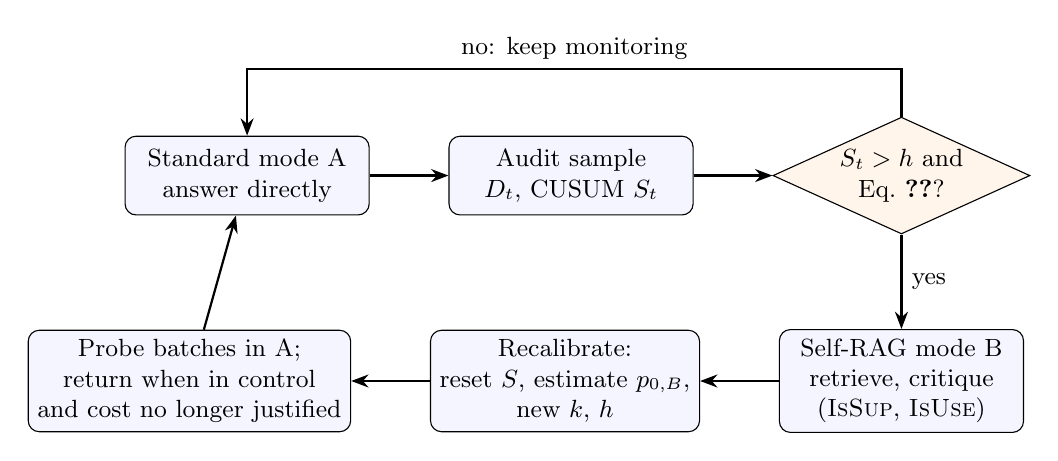
\begin{tikzpicture}[node distance=7mm and 10mm, every node/.style={font=\small},
 box/.style={draw, rounded corners, align=center, minimum width=31mm, minimum height=10mm, fill=blue!4},
 dec/.style={draw, diamond, aspect=2.2, align=center, inner sep=1pt, fill=orange!8},
 arr/.style={-{Stealth[length=2.2mm]}, thick}]
\node[box] (a) {Standard mode A\\answer directly};
\node[box, right=of a] (m) {Audit sample\\$D_t$, CUSUM $S_t$};
\node[dec, right=of m] (q) {$S_t>h$ and\\Eq.~\ref{eq:switch}?};
\node[box, below=12mm of q] (b) {Self-RAG mode B\\retrieve, critique\\(\tok{IsSup}, \tok{IsUse})};
\node[box, left=of b] (r) {Recalibrate:\\reset $S$, estimate $p_{0,B}$,\\new $k$, $h$};
\node[box, left=of r] (p) {Probe batches in A;\\return when in control\\and cost no longer justified};
\draw[arr] (a) -- (m);
\draw[arr] (m) -- (q);
\draw[arr] (q.north) -- ++(0,6mm) -| node[pos=0.25,above]{no: keep monitoring} (a.north);
\draw[arr] (q) -- node[right]{yes} (b);
\draw[arr] (b) -- (r);
\draw[arr] (r) -- (p);
\draw[arr] (p) -- (a);
\end{tikzpicture}
\caption{Proposed closed loop (ultimate research goal; not yet implemented). A small persistent shift detected by the CUSUM switches the model into Self-RAG mode when the cost criterion is met; the chart is then recalibrated for the new mode.}
\label{fig:loop}
\end{figure}

\begin{algorithm}[!htbp]
\caption{CUSUM-triggered Self-RAG (proposed)}\label{alg:loop}
\small
\begin{algorithmic}[1]
\State Phase I in mode A: estimate $p_{0,A}$; set $k_A$ from Eq.~\ref{eq:k}; choose $h_A$ by simulation for target ARL$_0$
\State mode $\gets$ A;\quad $S\gets 0$
\For{each batch $t$}
  \State generate responses in current mode; audit a sample; compute $D_t$, $\bar c_t$, $\bar\ell_t$
  \State $S\gets\max(0,\,S+D_t-k_{\text{mode}})$
  \If{mode $=$ A \textbf{and} $S>h_A$}
     \If{Eq.~\ref{eq:switch} holds \textbf{and} $\ell_B\le\ell_{\max}$}
        \State mode $\gets$ B;\quad log intervention;\quad run short Phase I in B to estimate $p_{0,B}$
        \State set $k_B$, $h_B$;\quad $S\gets 0$
     \Else
        \State alert human reviewer
     \EndIf
  \ElsIf{mode $=$ B}
     \State every $m$ batches run a probe batch in A and update probe CUSUM $S^{\mathrm{probe}}$
     \If{$S^{\mathrm{probe}}\le h_A$ for $r$ consecutive probes \textbf{and} Eq.~\ref{eq:switch} fails}
        \State mode $\gets$ A;\quad log intervention;\quad $S\gets 0$
     \EndIf
  \EndIf
\EndFor
\end{algorithmic}
\end{algorithm}

%=====================================================================
\section{Discussion}
\subsection{What the pilot shows}
Claim-level auditing against a verified answer key worked across three different SPC tasks, and its output, one binary label per response, feeds directly into standard monitoring statistics. The CUSUM accumulates repeated small excesses, so Gemini's recurring loan error appears as a steady climb; the EWMA weights recent batches, so Claude's single poor first batch triggers a signal that then fades; the LPRI keeps missing responses visible alongside defects. The most useful single finding is substantive: one counting error near a control limit recurred across sessions and across two of three model families. A benchmark score would average such an error away; a monitored, claim-level measurement system exposes it.

\subsection{Why the signals are not yet findings}
Five batches per model cannot estimate an in-control defect rate, and with batches of three a single defect moves $D_t$ by one third. Gemini's Run~5 verdict changes under three of four reasonable analyst choices. The run order is the order of recording, not a verified time order. The measurement system is not yet qualified: the audit was unblinded, GPT was self-evaluated, and repeatability and reproducibility are unmeasured. Batch independence and stationarity were not tested, and provider-side routing or silent updates could violate both.

\subsection{What a confirmatory study needs}
\begin{enumerate}[leftmargin=*]
\item \textbf{A qualified measurement system}: the Section~\ref{sec:kappa} study completed, with $\kappa\ge0.60$.
\item \textbf{A frozen process definition}: API access with fixed model identifier, system prompt, temperature and top-$p$; a provider timestamp on every response; any model or prompt change treated as an intervention that restarts the chart.
\item \textbf{Larger batches and recorded opportunities}: a rotating task pool of 6--10 prompts per batch, with the number of audited claims recorded so that DPMO can be reported.
\item \textbf{A Phase~I baseline}: at least 20--25 batches per model, checked for stability. With 75 responses at a true rate of 10\%, $p_0$ would still carry a 95\% interval of roughly 4--18\%.
\item \textbf{Designed limits}: $k$ from the estimated $p_0$ and a pre-stated $p_1$, then $h$ (and EWMA $L$) chosen by simulation for a target in-control ARL, reported under parameter uncertainty.
\item \textbf{A validated LPRI}: a test of whether it orders responses as expert raters do before it is given any deployability meaning.
\end{enumerate}

\subsection{Implications for industrial users}
A quality team using an LLM for SPC calculations should treat the model, version, prompt and settings as process metadata, keep an independent answer key for recurring tasks, and check classifications near a limit with particular care. The loan reanalysis is a reminder that human analyses need the same scrutiny: a phase defined too coarsely produced seven apparent violations that disappear once the data are split at the recorded interventions.

\section{Limitations}
The response archive is small (42 cleanly mapped of 45 planned) and incomplete. Model build identifiers, sampling settings and true timestamps were not logged. Labels come from one unblinded LLM audit with GPT self-evaluated, and the measurement system's accuracy and precision are not yet established. All chart parameters and LPRI weights are illustrative, and the five-run sequences are not verified time series. Only three datasets and one prompt per dataset were used. The closed loop of Section~\ref{sec:goal} is a proposal; its costs, latencies and benefits are untested. On the process side, forklift exposure, yield specifications and the meaning of the second loan column are unknown.

\section{Conclusion}
LLMs make analytical errors and hallucinate often enough, and confidently enough, that their analytical output needs to be measured the way industry measures any process it depends on. This paper sets out such a measurement system, states what it would take for it to be accurate, precise and credible, and couples it to a process-performance metric monitored with CUSUM and EWMA charts. In a pilot on DMAIC project data the system ran end to end, exposed a counting error that recurred across sessions and models, and produced chart signals whose operating properties can be stated exactly. Those signals are not yet evidence of drift or of any model's superiority; that requires the pre-specified rating study and a Phase~I baseline. The longer-term aim is a self-correcting loop in which a detected shift, and only a detected shift, buys the extra cost of retrieval and self-critique.

\section*{Declarations}
\textbf{Data and materials.} The process-data workbook, the three prompts, the response-level audit labels, the analysis code and the blank rater form are available at \url{https://github.com/srijabhattacharyya/LLM-SPC-Reliability}. The 43 response transcripts and the blinding key will be released after the blinded rating study, so that raters cannot identify which model produced each coded response.\\
\textbf{Use of AI tools.} The original response audit was performed with ChatGPT. Claude (Anthropic) assisted with manuscript drafting and with re-checking calculations in code. The author designed the study, collected the responses and is responsible for all content.\\
\textbf{Conflicts of interest.} None declared. No model provider was involved in the study.\\
\textbf{Funding.} None.\\
\textbf{Acknowledgements.} The author thanks Dr Subrata Rath, Head of the SQC \& OR Unit, Indian Statistical Institute, Pune, for guidance throughout this work.

\begin{thebibliography}{99}\small
\bibitem[AIAG(2010)]{aiag2010msa} Automotive Industry Action Group (2010). \emph{Measurement Systems Analysis Reference Manual} (4th ed.). AIAG. ISBN 978-1-60534-211-5.
\bibitem[Asai et~al.(2024)]{asai2024selfrag} Asai, A., Wu, Z., Wang, Y., Sil, A., \& Hajishirzi, H. (2024). Self-RAG: Learning to retrieve, generate, and critique through self-reflection. In \emph{The Twelfth International Conference on Learning Representations (ICLR 2024)}. arXiv:2310.11511.
\bibitem[Byrt et~al.(1993)]{byrt1993} Byrt, T., Bishop, J., \& Carlin, J. B. (1993). Bias, prevalence and kappa. \emph{Journal of Clinical Epidemiology}, 46(5), 423--429. \doi{10.1016/0895-4356(93)90018-V}
\bibitem[Chen et~al.(2024)]{chen2024chatgpt} Chen, L., Zaharia, M., \& Zou, J. (2024). How is ChatGPT's behavior changing over time? \emph{Harvard Data Science Review}, 6(2). \doi{10.1162/99608f92.5317da47}
\bibitem[Cobbe et~al.(2021)]{cobbe2021gsm8k} Cobbe, K., Kosaraju, V., Bavarian, M., Chen, M., Jun, H., Kaiser, L., Plappert, M., Tworek, J., Hilton, J., Nakano, R., Hesse, C., \& Schulman, J. (2021). Training verifiers to solve math word problems. arXiv:2110.14168.
\bibitem[Cohen(1960)]{cohen1960} Cohen, J. (1960). A coefficient of agreement for nominal scales. \emph{Educational and Psychological Measurement}, 20(1), 37--46.
\bibitem[Cohen(1968)]{cohen1968} Cohen, J. (1968). Weighted kappa: Nominal scale agreement with provision for scaled disagreement or partial credit. \emph{Psychological Bulletin}, 70(4), 213--220.
\bibitem[Crosier(1988)]{crosier1988} Crosier, R. B. (1988). Multivariate generalizations of cumulative sum quality-control schemes. \emph{Technometrics}, 30(3), 291--303.
\bibitem[Feinstein and Cicchetti(1990)]{feinstein1990} Feinstein, A. R., \& Cicchetti, D. V. (1990). High agreement but low kappa: I. The problems of two paradoxes. \emph{Journal of Clinical Epidemiology}, 43(6), 543--549. \doi{10.1016/0895-4356(90)90158-L}
\bibitem[Fleiss(1971)]{fleiss1971} Fleiss, J. L. (1971). Measuring nominal scale agreement among many raters. \emph{Psychological Bulletin}, 76(5), 378--382.
\bibitem[Gama et~al.(2014)]{gama2014survey} Gama, J., \v{Z}liobait\.{e}, I., Bifet, A., Pechenizkiy, M., \& Bouchachia, A. (2014). A survey on concept drift adaptation. \emph{ACM Computing Surveys}, 46(4), Article 44. \doi{10.1145/2523813}
\bibitem[Huang et~al.(2025)]{huang2025survey} Huang, L., Yu, W., Ma, W., Zhong, W., Feng, Z., Wang, H., Chen, Q., Peng, W., Feng, X., Qin, B., \& Liu, T. (2025). A survey on hallucination in large language models: Principles, taxonomy, challenges, and open questions. \emph{ACM Transactions on Information Systems}. \doi{10.1145/3703155}
\bibitem[Jensen et~al.(2006)]{jensen2006} Jensen, W. A., Jones-Farmer, L. A., Champ, C. W., \& Woodall, W. H. (2006). Effects of parameter estimation on control chart properties: A literature review. \emph{Journal of Quality Technology}, 38(4), 349--364. \doi{10.1080/00224065.2006.11918623}
\bibitem[Ji et~al.(2023)]{ji2023hallucination} Ji, Z., Lee, N., Frieske, R., Yu, T., Su, D., Xu, Y., Ishii, E., Bang, Y. J., Madotto, A., \& Fung, P. (2023). Survey of hallucination in natural language generation. \emph{ACM Computing Surveys}, 55(12), Article 248. \doi{10.1145/3571730}
\bibitem[Kalai et~al.(2025)]{kalai2025why} Kalai, A. T., Nachum, O., Vempala, S. S., \& Zhang, E. (2025). Why language models hallucinate. arXiv:2509.04664.
\bibitem[Lewis et~al.(2020)]{lewis2020rag} Lewis, P., Perez, E., Piktus, A., Petroni, F., Karpukhin, V., Goyal, N., K\"uttler, H., Lewis, M., Yih, W., Rockt\"aschel, T., Riedel, S., \& Kiela, D. (2020). Retrieval-augmented generation for knowledge-intensive NLP tasks. In \emph{Advances in Neural Information Processing Systems 33 (NeurIPS 2020)}. arXiv:2005.11401.
\bibitem[Liang et~al.(2023)]{liang2023helm} Liang, P., Bommasani, R., Lee, T., et~al. (2023). Holistic evaluation of language models. \emph{Transactions on Machine Learning Research}. \url{https://openreview.net/forum?id=iO4LZibEqW}
\bibitem[Lin et~al.(2022)]{lin2022truthfulqa} Lin, S., Hilton, J., \& Evans, O. (2022). TruthfulQA: Measuring how models mimic human falsehoods. In \emph{Proceedings of the 60th Annual Meeting of the Association for Computational Linguistics (Volume 1: Long Papers)}, 3214--3252. \doi{10.18653/v1/2022.acl-long.229}
\bibitem[Lowry et~al.(1992)]{lowry1992} Lowry, C. A., Woodall, W. H., Champ, C. W., \& Rigdon, S. E. (1992). A multivariate exponentially weighted moving average control chart. \emph{Technometrics}, 34(1), 46--53. \doi{10.2307/1269551}
\bibitem[Lucas and Saccucci(1990)]{lucas1990} Lucas, J. M., \& Saccucci, M. S. (1990). Exponentially weighted moving average control schemes: Properties and enhancements. \emph{Technometrics}, 32(1), 1--12. \doi{10.2307/1269835}
\bibitem[Manakul et~al.(2023)]{manakul2023selfcheckgpt} Manakul, P., Liusie, A., \& Gales, M. (2023). SelfCheckGPT: Zero-resource black-box hallucination detection for generative large language models. In \emph{Proceedings of the 2023 Conference on Empirical Methods in Natural Language Processing}, 9004--9017. \doi{10.18653/v1/2023.emnlp-main.557}
\bibitem[Min et~al.(2023)]{min2023factscore} Min, S., Krishna, K., Lyu, X., Lewis, M., Yih, W., Koh, P. W., Iyyer, M., Zettlemoyer, L., \& Hajishirzi, H. (2023). FActScore: Fine-grained atomic evaluation of factual precision in long form text generation. In \emph{Proceedings of the 2023 Conference on Empirical Methods in Natural Language Processing}, 12076--12100. \doi{10.18653/v1/2023.emnlp-main.741}
\bibitem[Montgomery(2019)]{montgomery2019} Montgomery, D. C. (2019). \emph{Introduction to Statistical Quality Control} (8th ed.). Wiley.
\bibitem[NIST/SEMATECH(n.d.)]{nist} NIST/SEMATECH (n.d.). \emph{e-Handbook of Statistical Methods}, Section 6.3.2.3: CUSUM control charts. National Institute of Standards and Technology. \url{https://www.itl.nist.gov/div898/handbook/pmc/section3/pmc323.htm}
\bibitem[Page(1954)]{page1954} Page, E. S. (1954). Continuous inspection schemes. \emph{Biometrika}, 41(1/2), 100--115. \doi{10.1093/biomet/41.1-2.100}
\bibitem[Panickssery et~al.(2024)]{panickssery2024self} Panickssery, A., Bowman, S. R., \& Feng, S. (2024). LLM evaluators recognize and favor their own generations. In \emph{Advances in Neural Information Processing Systems 37 (NeurIPS 2024)}. arXiv:2404.13076.
\bibitem[Reynolds and Stoumbos(1999)]{reynolds1999} Reynolds, M. R., Jr., \& Stoumbos, Z. G. (1999). A CUSUM chart for monitoring a proportion when inspecting continuously. \emph{Journal of Quality Technology}, 31(1), 87--108. \doi{10.1080/00224065.1999.11979900}
\bibitem[Roberts(1959)]{roberts1959} Roberts, S. W. (1959). Control chart tests based on geometric moving averages. \emph{Technometrics}, 1(3), 239--250. \doi{10.1080/00401706.1959.10489860}
\bibitem[Zheng et~al.(2023)]{zheng2023judge} Zheng, L., Chiang, W.-L., Sheng, Y., Zhuang, S., Wu, Z., Zhuang, Y., Lin, Z., Li, Z., Li, D., Xing, E. P., Zhang, H., Gonzalez, J. E., \& Stoica, I. (2023). Judging LLM-as-a-judge with MT-Bench and Chatbot Arena. In \emph{Advances in Neural Information Processing Systems 36 (NeurIPS 2023), Datasets and Benchmarks Track}. arXiv:2306.05685.
\end{thebibliography}

\appendix
\section{Prompts used (verbatim)}\label{app:prompts}
Each prompt was pasted unchanged into a fresh chat.

\subsection*{A.1 Forklift breakdown}
\begin{quote}\small
You are participating in a research experiment evaluating the analytical reliability of large language models on industrial Six Sigma datasets. Analyse the following dataset independently. Do not assume that any conclusion is correct unless supported by the data. Do not invent missing information. If something cannot be established, explicitly say so.

Dataset: Forklift Breakdown. The observations represent the number of forklift breakdowns per 15-day period.\\
Baseline (15 observations): [3, 9, 8, 7, 2, 3, 6, 2, 5, 4, 3, 5, 5, 6, 3]\\
Analyse \& Improve (19 observations): [1, 3, 0, 7, 4, 5, 3, 9, 2, 1, 5, 5, 11, 4, 0, 3, 0, 5, 6]\\
Control (13 observations): [2, 1, 1, 4, 1, 0, 1, 3, 1, 2, 0, 1, 1]\\
The operational target is strictly fewer than 3 breakdowns per 15-day period.

Answer these questions: (1) Verify the number of observations in each phase. (2) Calculate the mean, median, sample standard deviation, minimum and maximum for each phase. (3) Calculate the percentage reduction in mean breakdowns from Baseline to Control. (4) Calculate the proportion of periods meeting the target in each phase. Remember that exactly 3 does NOT meet a strictly-less-than-3 target. (5) Identify unusual observations or possible anomalies. (6) Select an appropriate control chart and justify your selection. (7) Calculate the Baseline c-chart centre line, UCL and LCL, showing the formula and calculations. (8) Discuss whether a Poisson assumption is reasonable. Distinguish a preliminary diagnostic from a formal goodness-of-fit conclusion. (9) Explain whether the process can be considered statistically stable. Do not equate improvement with stability. (10) Identify limitations and any information that is missing.

Output format: a table of phase-wise descriptive statistics; a table of target achievement; control-chart calculations; a short interpretation; a list of limitations. Show numerical calculations. Do not fabricate DPMO, opportunities, p-values, or other missing values.
\end{quote}

\subsection*{A.2 Manufacturing yield}
\begin{quote}\small
You are participating in a research experiment evaluating the analytical reliability of large language models on industrial Six Sigma datasets. Analyse the following dataset independently. Do not invent missing information or assume that correlation proves causation.

Dataset: Manufacturing Yield. The observations represent percentage yield across individual production experiments.\\
Baseline (10 observations): [7.1, 6.9, 7.2, 6.8, 7.2, 6.8, 6.7, 7.1, 7.0, 7.3]\\
Improve (8 observations): [8.5, 8.7, 8.9, 8.8, 8.4, 8.7, 8.8, 9.0]\\
Control (7 observations): [9.8, 10.0, 9.9, 10.0, 9.8, 9.9, 10.1]

Answer these questions: (1) Verify the sample size in each phase. (2) Calculate the mean, median, sample standard deviation, minimum and maximum for each phase. (3) Calculate the absolute increase in mean yield from Baseline to Control in percentage points. (4) Calculate the relative percentage increase from Baseline to Control. (5) Compare variability across the three phases. (6) Recommend an appropriate control chart and explain the assumptions required. (7) Explain whether process capability indices Cp and Cpk can be calculated from the supplied data. If not, explain exactly what is missing. (8) Discuss whether the observed phase differences establish that the improvement interventions caused the yield increase. (9) Identify what further information would be required for a stronger statistical analysis. (10) State the limitations of your conclusions.

Output format: a table of phase-wise descriptive statistics; calculations for the Baseline-to-Control change; recommended statistical methods; a short interpretation and limitations. Show your calculations. Do not invent specification limits, p-values, intervention details, or causal explanations.
\end{quote}

\subsection*{A.3 Loan disbursement days}
\begin{quote}\small
You are participating in a research experiment evaluating the analytical reliability of large language models on industrial and service-quality datasets. Analyse the following monthly loan-disbursement dataset independently. Do not invent missing information or make unsupported causal claims.

Dataset: Loan Disbursement Days.\\
Baseline (26 observations): [23,\allowbreak{}22,\allowbreak{}21,\allowbreak{}17,\allowbreak{}16,\allowbreak{}21,\allowbreak{}21,\allowbreak{}19,\allowbreak{}20,\allowbreak{}19,\allowbreak{}23,\allowbreak{}18,\allowbreak{}21,\allowbreak{}23,\allowbreak{}20,\allowbreak{}25,\allowbreak{}26,\allowbreak{}18,\allowbreak{}25,\allowbreak{}19,\allowbreak{}18,\allowbreak{}17,\allowbreak{}22,\allowbreak{}19,\allowbreak{}20,\allowbreak{}19]\\
Analyse \& Improve (36 observations): [11,\allowbreak{}12,\allowbreak{}14,\allowbreak{}11,\allowbreak{}13,\allowbreak{}14,\allowbreak{}12,\allowbreak{}11,\allowbreak{}11,\allowbreak{}12,\allowbreak{}14,\allowbreak{}11,\allowbreak{}11,\allowbreak{}11,\allowbreak{}9,\allowbreak{}11,\allowbreak{}9,\allowbreak{}9,\allowbreak{}10,\allowbreak{}9,\allowbreak{}9,\allowbreak{}11,\allowbreak{}11,\allowbreak{}12,\allowbreak{}10,\allowbreak{}8,\allowbreak{}7,\allowbreak{}7,\allowbreak{}8,\allowbreak{}8,\allowbreak{}7,\allowbreak{}8,\allowbreak{}7,\allowbreak{}8,\allowbreak{}9,\allowbreak{}10]\\
Control (7 observations): [7,\allowbreak{}8,\allowbreak{}7,\allowbreak{}7,\allowbreak{}8,\allowbreak{}7,\allowbreak{}8]\\
The values represent the number of days required to disburse loans. The workbook also records these improvement annotations: December 2021: Automation of document collection and verification through a government portal. December 2022: Use of an independent loan assessor/property evaluator. December 2023: Aadhaar-based verification of civil score.

Answer these questions: (1) Verify the sample size in each phase. (2) Calculate the mean, median, sample standard deviation, minimum and maximum for each phase. (3) Calculate the absolute and relative reduction in mean disbursement time from Baseline to Control. (4) Recommend an appropriate control chart and explain why. (5) Calculate Individuals chart limits using the moving-range method separately for each phase. Use: I-chart limits = mean $\pm$ 2.66 $\times$ average moving range; MR-chart UCL = 3.267 $\times$ average moving range; MR-chart LCL = 0. (6) Explain whether any observations exceed the calculated phase-specific limits. (7) Explain why phase-specific control limits do not establish that the entire process was stable across all phases. (8) Discuss whether the improvement annotations establish causation. (9) Identify missing or ambiguous information that limits analysis. (10) State your conclusions and limitations.

Show calculations. Do not invent application volumes, exposure denominators, p-values, or causal effects.
\end{quote}

\section{Scoring decision rules}
\begin{itemize}[leftmargin=*]
\item Score every factual or analytical claim against the Section~\ref{sec:reference} reference values.
\item Score 1 only for non-material issues such as rounding or wording.
\item Score 2 when an error changes a statistic, a threshold classification, a chart interpretation or a supported conclusion.
\item Score 3 for fabricated data, invented tests or results, or high-impact unsupported claims such as asserting that an intervention caused a change.
\item Label a response defective if any claim scores 2 or 3.
\item Record missing, duplicate, wrong-dataset and ambiguously mapped responses as data-integrity events, never as defects or valid trials.
\item Score final answers and shown working separately; a correct final answer reached through wrong working scores 1 with a working-error flag.
\end{itemize}

\section{Supplementary materials}
\begin{itemize}[leftmargin=*]
\item \textbf{S1.} Process-data workbook (three sheets; months and intervention notes for the loan data). Available in the repository.
\item \textbf{S2.} Response transcripts, coded R01--R43. To be released after the blinded rating study.
\item \textbf{S3.} Blinded rating kit: rater form (available in the repository); master workbook with blinding key, adjudication sheet and agreement calculator (held by the author until the rating study is complete).
\item \textbf{S4.} Analysis scripts: reference values, CUSUM/EWMA series, sensitivity analyses, ARL simulation, figures, and $\kappa$ with bootstrap intervals. Available in the repository.
\end{itemize}

\end{document}
